\begin{document}

\def\title{Final Review Session}

\newcommand{\qitem}{\qpart\item}

\renewcommand{\labelenumi}{(\alph{enumi})} % change default enum format to (a)
\renewcommand{\theenumi}{(\alph{enumi})} % fix reference format accordingly.
\renewcommand{\labelenumii}{\roman{enumii}.} % second level labels.
\renewcommand{\theenumii}{\roman{enumii}.}

\maketitle

\vspace{0.5em}

\section{Module 1}
\section*{Midterm 1 Review}

\renewcommand{\arraystretch}{1.25}

\subsection*{Transistors}

\begin{center} 
\begin{tabular}[t]{|c|c|p{200px}|}
\hline
Type & Drawing & Behavior \\ \hline
 \begin{minipage}[c]{30px} PMOS \end{minipage} & \begin{minipage}[c]{50px} \begin{circuitikz}[american] 
\draw (0, 0) node[pmos] (nmos) {};
\draw (nmos.G) node[left]{$G$};
\draw (nmos.S) node[left]{$S$};
\draw (nmos.D) node[left]{$D$};
\end{circuitikz}
\end{minipage} & 
\begin{minipage}[t]{200px}
\vspace{-22px}
Closed switch when gate voltage $V_G$ is at least $|V_{tp}|$ below source voltage $V_S$ (gate voltage is low). Open switch otherwise.
\end{minipage} \\ \hline
\begin{minipage}[c]{30px} NMOS \end{minipage} & 
\begin{minipage}[c]{50px}
\begin{circuitikz}[american] 
\draw (0, 0) node[nmos] (nmos) {};
\draw (nmos.G) node[left]{$G$};
\draw (nmos.S) node[left]{$S$};
\draw (nmos.D) node[left]{$D$};
\end{circuitikz}
\end{minipage} & 

\begin{minipage}[t]{200px}
\vspace{-22px}
Closed switch when gate voltage $V_G$ is at least $V_{tn}$ above source voltage $V_S$ (gate voltage is high). Open switch otherwise.
\end{minipage} \\ \hline
\end{tabular} \end{center}

\begin{center} \begin{tabular}{|c|c|c|c|}
\hline
Type & (Voltage-Controlled) Switch & Resistor-Switch & Resistor-Capacitor-Switch \\ \hline
\begin{minipage}[c]{30px} \vspace{-110px} PMOS \end{minipage}
 & \begin{circuitikz}[scale=0.9]
			\draw (0, -2) node[label=left:$D$] {}
			to[switch, l_= $V_{GS} \leq -|V_{tp}|$, *-] (0,2)
			to[short, -*] ++(0, 0.2)
            node[label=right:$S$] {};;
			\draw (0, 2) -- (-1, 2)
			to[short, -*] ++(0, -2) node[label=left:$G$] {};;
			\draw (0, -1.75) to [short, -*, l=$V_{out}$] ++(1,0);;
		\end{circuitikz} & 
        \begin{circuitikz}[scale=0.9]
			\draw (0, -2) node[label=left:$D$] {}
			to[switch,l_= $V_{GS} \leq -|V_{tp}|$, *-] (0,0)
			to[R, l_=$R_{on}$, i<=$I_D$] ++(0, 2)
			to[short, -*] ++(0, 0.2) node[label=right:$S$] {};;
			\draw (0, 2) -- (-1, 2)
			to[short, -*] ++(0, -2) node[label=left:$G$] {};;
			\draw (0, -1.75) to [short, -*, l=$V_{out}$] ++(1,0);;
		\end{circuitikz} &
        \begin{circuitikz}[scale=0.9]
			\draw (0, -2) node[label=left:$D$] {}
			to[switch,l_= $V_{GS} \leq -|V_{tp}|$, *-] (0,0)
			to[R, l_=$R_{on}$, i<=$I_D$] ++(0, 2)
			to[short, -*] ++(0, 0.2)
            node[label=right:$S$] {};;
			\draw (0, 2) -- (-1, 2)
			to[C, -*, l_=$C_{GS}$] ++(0, -2) node[label=left:$G$] {};;
			\draw (0, -1.75) to [short, -*, l=$V_{out}$] ++(1,0);;
		\end{circuitikz} \\ \hline

\begin{minipage}[c]{30px} \vspace{-110px} NMOS \end{minipage}
 & \begin{circuitikz}[scale=0.9]
            \draw (0,-2)
            to[switch,l_= $V_{GS} \geq V_{tn}$]
            (0,2) to[short, -*] ++(0,0)
            node[label=left:$D$] {};;
            \draw (0,-2) -- (-1,-2)
            to[short, -*] ++(0,2) node[label=left:$G$] {};;
            \draw (0,1.75) to [short,-*,l=$V_{out}$] ++ (1,0);;
            \draw (0, -2) to [short, -*] ++(0, -0.2) node[label=right:$S$] {};;
        \end{circuitikz} &
        \begin{circuitikz}[scale=0.9]
            \draw (0,-2)
            to[switch,l_= $V_{GS} \geq V_{tn}$]
            (0,0) to[R,-*,l=$R_{on, N}$,i<=$I_D$] ++(0,2)
            node[label=left:$D$] {};;
            \draw (0,-2) -- (-1,-2)
            to[short, -*] ++(0,2) node[label=left:$G$] {};;
            \draw (0,1.75) to [short,-*,l=$V_{out}$] ++ (1,0);;
            \draw (0, -2) to [short, -*] ++(0, -0.2) node[label=right:$S$] {};;
        \end{circuitikz} & 
        \begin{circuitikz}[scale=0.9]
            \draw (0,-2)
            to[switch,l_= $V_{GS} \geq V_{tn}$]
            (0,0) to[R,-*,l=$R_{on, N}$,i<=$I_D$] ++(0,2)
            node[label=left:$D$] {};;
            \draw (0,-2) -- (-1,-2)
            to[C,-*,l=$C_{GS}$] ++(0,2) node[label=left:$G$] {};;
            \draw (0,1.75) to [short,-*,l=$V_{out}$] ++ (1,0);;
            \draw (0, -2) to [short, -*] ++(0, -0.2) node[label=right:$S$] {};;
        \end{circuitikz} \\ \hline
\end{tabular} \end{center}

\subsection*{First-Order Differential Equations}
\begin{enumerate}
    \item \textbf{Homogeneous Case}: the first derivative of the state variable $x(t)$ is proportional to the state variable by some constant $\lambda$. The general form of a homogeneous differential equation is:
    \begin{align*}
        \boxed{\frac{d}{dt} x(t) = \lambda x(t)}
    \end{align*}
    Given some initial state $x(0)$, the unique solution to this differential equation is:
    \begin{align*}
        \boxed{x(t) = x(0) e^{\lambda t}}
    \end{align*}

    \item \textbf{Non-homogenous Case}: the first derivative of the state variable $x(t)$ is equal to a scaled multiple of the state plus a nonzero constant. The general form of a non-homogeneous differential equation is:
    \begin{align*}
        \boxed{\frac{d}{dt} x(t) = \lambda x(t) + \alpha}
    \end{align*}
    To solve this type of differential equation, use a change of variables $x(t) = z(t) - \frac{\alpha}{\lambda}$. Plugging in this new definition of $x(t)$ into the original differential equation, we get the homogeneous case with respect to the new variable $z(t)$:
    \begin{align*}
        \frac{d}{dt} x(t) &= \lambda x(t) + \alpha \\
        \frac{d}{dt} (z(t) - \frac{\alpha}{\lambda}) &= \lambda (z(t) - \frac{\alpha}{\lambda}) + \alpha \\
        \frac{d}{dt} z(t) &= \lambda z(t)
    \end{align*}
    Now, you can use the result from the homogenous case to solve the differential equation in terms of $z(t)$, and then change variables back to $x(t)$ to get your final solution.
    \begin{align*}
        z(t) &= z(0) e^{\lambda t} \\
        x(t) + \frac{\alpha}{\lambda} &= (x(0) + \frac{\alpha}{\lambda}) e^{\lambda t} \\
    \end{align*}

    \vspace{-35px}
    $$\boxed{x(t) = x(0) e^{\lambda t} + \frac{\alpha}{\lambda}(e^{\lambda t} - 1)}$$

    \item \textbf{Non-homogeneous with Nonconstant Input $u(t)$}: the first derivative of the state variable is equal to a scalar multiple of the state plus a general non-constant function $u(t)$.
    \begin{align*}
        \boxed{\frac{d}{dt} x(t) = \lambda x(t) + u(t)}
    \end{align*}
    The solution to this differential equation is:
    \begin{align*}
        \boxed{x(t) = x(0) e^{\lambda t} + \int_0^t u(\tau) e^{\lambda(t - \tau)} \, d\tau}
    \end{align*}
\end{enumerate}
\newpage 
\subsection*{Time-Domain RC circuits}
\begin{figure}[H]
	\begin{center}
		\begin{circuitikz}
			\draw (0, 4)
			to[V =$V_s$] (0, 0);
			\draw (0, 4)
			to[switch,l^=\mbox{$t = 0$}](3,4)
			(3,4) to[R = $R$,v=$V_R(t)$,i>^=$i_R(t)$] (6,4)	
			to [short] (8,4)
			to[C = $C$, v=$V_{C}(t)$,i>^=$i_C(t)$] (8,0)
			to [short] (0,0);
		\end{circuitikz}
		\caption{\label{fig:circuit}RC Circuit with Voltage Source}
	\end{center}
\end{figure}

\begin{enumerate}
    \item \textbf{Step 1}: Use KCL and KVL equations, and the capacitor charge-voltage relationship $i_C(t) = C \frac{d}{dt} V_C(t)$ to get a differential equation in terms of the given variable (typically $V_C(t)$ or $i_C(t)$).
    
    For the above circuit, KCL gives us the following differential equation:
    \begin{align*}
        i_R(t) &= i_C(t) \\
        \frac{V_s - V_C(t)}{R} &= C \frac{d}{dt} V_C(t)
    \end{align*}

    \item \textbf{Step 2}: Identify the differential equation as homogenous, non-homogenous, or having a non-constant input, and solve the differential equation using the tools above.

    We can express the above differential equation the form:
    \begin{align*}
        \frac{d}{dt} V_C(t) = -\frac{1}{RC} V_C(t) + \frac{1}{RC} V_s
    \end{align*}

    How would you solve this differential equation if $V_s = 0$? $V_s = V_{DD} > 0$? $V_s(t) = e^{-t}$?

    \item \textbf{Step 3}: Plug initial conditions into your solution.

    For example, uncharged capacitors have an initial condition $V_C(t = 0) = 0$.
\end{enumerate}

Note: Circuits with inductors can be solved in a similar manner, using the inductor I-V relationship: 
$$\boxed{V_L(t) = L \frac{d}{dt} i_L(t)}$$

\newpage
\subsection*{Diagonalization and Change of Basis}

We start with a system of the form with a diagonalizable $n \times n$ matrix $A$:
\begin{align*}
    \vec{y} = A \vec{x}
\end{align*}
We can find the eigenvalues $\lambda_1, \lambda_2, \ldots, \lambda_n$ and eigenvectors $\vec{v}_1, \vec{v}_2, \ldots \vec{v}_n$. The eigenbasis is this set of $n$ eigenvectors that spans $\mathbb{R}^n$, with the eigenbasis matrix defined below:
\begin{align*}
    V = \begin{bmatrix}
        \vec{v_1} & \vec{v_2} & \dots & \vec{v_n}
    \end{bmatrix}
\end{align*}

Given this definition of $V$, we can express any vector $\vec{x} \in \mathbb{R}^n$ as a linear combination of eigenvectors of $A$:
\begin{align*}
    \vec{x} = \alpha_1 \vec{v_1} + \alpha_2 \vec{v_2} + \dots + \alpha_n \vec{v_n} = V \begin{bmatrix} \alpha_1 \\ \vdots \\ \alpha_n \end{bmatrix} = V \vec{\widetilde{x}}
\end{align*}
We define the coordinates of $\vec{x}$ in the eigenbasis as the vector of $\alpha_i$'s, which we represent as $\vec{\widetilde{x}}$. The following relationships define changing from the eigenbasis coordinate system:
\begin{align*}
    \vec{x} = V \vec{\widetilde{x}} \\
    \vec{\widetilde{x}} = V^{-1} \vec{x}
\end{align*}

Then, if we substitute $\vec{x} = V \vec{\widetilde{x}}$ and $\vec{y} = V \vec{\widetilde{y}}$ in the original system, we get
\begin{align*}
    V \vec{\widetilde{y}} &= AV \vec{\widetilde{x}} \\
    \vec{\widetilde{y}} &= V^{-1}AV \vec{\widetilde{x}} \\
    \vec{\widetilde{y}} &= \Lambda \vec{\widetilde{x}}
\end{align*}

Because $V$ is the eigenbasis, $V^{-1}AV$ is the matrix $\Lambda$ with the eigenvalues on the diagonal:
\begin{align*}
    \boxed{\Lambda = V^{-1}AV} = 
    \begin{bmatrix}
        \lambda_1 & 0 & \dots & 0 \\
        0 & \lambda_2 & \dots & 0 \\
        \vdots & \vdots & \ddots & \vdots \\
        0 & 0 & \dots & \lambda_n
    \end{bmatrix}
\end{align*}

Thus, the diagonalization of $\boxed{A = V \Lambda V^{-1}}$. You may find this diagram useful to visualize this process, where the $V^{-1}$ brings a vector into the eigenbasis, $\Lambda$ represents $A$'s linear transformation in the eigenbasis coordaintes, and $V$ brings the vector back into standard coordinates.
\begin{figure}[H]
    \centering
    \begin{tikzpicture}[node distance = 1.5cm, thick, every node/.style={inner sep=0.25em,outer sep=0.25em}]%
      \node (1) [circle,draw,minimum size=2em] {$\vec{x}$};
      \node (2) [circle,draw,right=of 1,minimum size=2em] {$\vec{y}$};
      \node (3) [circle,draw,below=of 2,minimum size=2em] {$\vec{\widetilde{y}}$};
      \node (4) [circle,draw,below=of 1,minimum size=2em] {$\vec{\widetilde{x}}$};
      \draw[->] (1) -- node [draw,midway,above] {$A$} (2);
      \draw[->] (1.240) -- node [draw,midway,left]{$V^{-1}$} (4.120);
      \draw[->] (4.60) -- node [draw,midway,right]{$V$} (1.300);
      \draw[->] (2.300) -- node [draw,midway,right]{$V^{-1}$} (3.60);
      \draw[->] (3.120) -- node [draw,midway,left]{$V$} (2.240);
      \draw[->] (4) -- node [,draw,midway,below] {$\Lambda$} (3);
    \end{tikzpicture}
\end{figure}

\subsection*{Multivariate Differential Equations}
Consider a system of differential equations of the form:
\begin{align*}
    \frac{d}{dt} \vec{x}(t) = A \vec{x}(t)
\end{align*}

The strategy is to diagonalize the system so that there is a set of $n$ separate first order homogeneous differential equations that we can solve individually and recover the solutions in the original coordinates.

\begin{enumerate}
    \item \textbf{Step 1}: Find the eigenvalue-eigenvector pairs $(\lambda_1, \vec{v_1}), \dots (\lambda_n, \vec{v_n})$ of your $A$ matrix.

    \item \textbf{Step 2}: Define $V = \begin{bmatrix}
        \vec{v_1} & \vec{v_2} & \dots & \vec{v_n}
    \end{bmatrix}$, $\vec{x}(t) = V \vec{\widetilde{x}}(t)$, and transform your system to eigenbasis coordinates.

    \begin{align*}
    \frac{d}{dt} \vec{\widetilde{x}}(t) &=  V^{-1}AV \vec{\widetilde{x}}(t) =
    \begin{bmatrix}
        \lambda_1 & 0 & \dots & 0 \\
        0 & \lambda_2 & \dots & 0 \\
        \vdots & \vdots & \ddots & \vdots \\
        0 & 0 & \dots & \lambda_n
    \end{bmatrix} \vec{\widetilde{x}}(t) \\
    \vec{\widetilde{x}}(0) &= V^{-1} \vec{x}(0)
    \end{align*}

    \item \textbf{Step 3}: We can then decompose this diagonal matrix-vector equation into $n$ single-variable differential equations:
    \begin{align*}
        \frac{d}{dt} \widetilde{x_1}(t) &= \lambda_1 \widetilde{x_1}(t) \\
        &\vdots \\
        \frac{d}{dt} \widetilde{x_n}(t) &= \lambda_n \widetilde{x_n}(t)
    \end{align*}

    \item \textbf{Step 4}: Solve each equation to get expressions for $\widetilde{x}_1(t), \ldots \widetilde{x}_n(t)$.
    \begin{align*}
        \widetilde{x_1}(t) &= \widetilde{x_1}(0) e^{\lambda_1 t} \\
        &\vdots \\
        \widetilde{x_n}(t) &= \widetilde{x_1}(0) e^{\lambda_n t} 
    \end{align*}

    \item \textbf{Step 5}: Transform your solution back to the standard basis coordinates.
    \begin{align*}
        \vec{x}(t) = V \vec{\widetilde{x}}(t)
    \end{align*}
\end{enumerate}

\textbf{Second-Order ODE}: If we have a differential equation that depends on $\frac{d^2}{dt^2} x(t)$, define your state vector as $\begin{bmatrix} x(t) & \frac{d}{dt} x(t) \end{bmatrix}^T$ and solve your system as a multivariate differential equation.

\textbf{Complex Eigenvalues}: The behavior of a system (for example, a RLC circuit) in the time domain varies based on whether its eigenvalues are real, imaginary, or complex.
\begin{enumerate}
    \item \textbf{Purely Real Eigenvalues ($\lambda = a$)}: The time-domain response is a decaying exponential with no oscillations.
    \item \textbf{Purely Imaginary Eigenvalues ($\lambda = bj$)}: The response is a sinusoid that oscillates without decaying.
    \item \textbf{Complex Eigenvalues ($\lambda = a + bj$)}: The response is the product of a decaying exponential and a sinusoid, so it oscillates as it decays.
\end{enumerate}

\newpage
\subsection*{Complex Numbers}
\textbf{Complex Number Representations:} 

\hspace{2 em} Rectangular Form: $z = a + bj$ \hspace{14em} Polar Form: $z = re^{j\theta}$

\begin{figure}[h]
\centering
    \begin{tikzpicture}[scale=0.8, transform shape]
    \draw (0,-4)--(0,4) node[above] {$Im$} (-4,0)--(4,0) node[right] {$Re$};
    \draw[dashed] (0,0) circle (3) circle (2) circle (1);
    \draw (-1.15,0.93)--(-1.15,1.045) node[near start, fill=white] {$r = 1$};
    \draw (-1.85,1.65)--(-1.78,1.78) node[near start=3pt, fill=white] {$r = 2$};
    \draw (-2.45,2.45)--(-2.55,2.55) node[near start=3pt, fill=white] {$r = 3$};
    \draw [line width=0.25mm, blue, ->] (0,0) -- (2.4,1.3) node [below right] {};
    \draw [dotted, line width=0.25mm, blue, ->] (0,0) -- (2.4,0) node [below right]{};
    \draw [dotted, line width=0.25mm, blue, ->] (2.4,0) -- (2.4,1.3) node [below right]{};
    \draw (1.5,-0.3)--(1.6,-0.3) node[near start=3pt, fill=white] {\color{blue}$a$};
    \draw (2.7,0.6)--(2.7,0.6) node[near start=3pt, fill=white] {\color{blue}$b$};
    \draw (3.5,1.4)--(3.5,1.4) node[near start=3pt, fill=white] {\color{blue}$z = a + bj$};
    \end{tikzpicture}
\hfill
    \begin{tikzpicture}[scale=0.8, transform shape]
    \draw (0,-4)--(0,4) node[above] {$Im$} (-4,0)--(4,0) node[right] {$Re$};
    \draw[dashed] (0,0) circle (3) circle (2) circle (1);
    \draw (-1.15,0.93)--(-1.15,1.045) node[near start, fill=white] {$r = 1$};
    \draw (-1.85,1.65)--(-1.78,1.78) node[near start=3pt, fill=white] {$r = 2$};
    \draw (-2.45,2.45)--(-2.55,2.55) node[near start=3pt, fill=white] {$r = 3$};
    \draw [line width=0.25mm, blue, ->] (0,0) -- (2.4,1.3) node [below right] {};
    \draw (3.2,1.55)--(3.2,1.55) node[near start=3pt, fill=white] {\color{blue}$z = r e^{j \theta}$};
    \draw (1.2,1.0)--(1.2,1.0) node[near start=3pt, fill=white] {\color{blue}$r$};
    \draw (0.6,0.15)--(0.6,0.15) node[scale=0.9,text opacity=1, opacity=0,near start=3pt, fill=white] {\color{blue}\small$\theta$};
    \end{tikzpicture}
\end{figure}

\textbf{Complex Conjugates:}
    \begin{align*}
        \boxed{\overline{a + bj} = a - bj} \hspace{30px} \boxed{\overline{re^{j\theta}} = re^{-j\theta}}
    \end{align*}

\textbf{Operations with Complex Numbers:}
\begin{enumerate}
    \item Rectangular to polar:
    \begin{align*}
        \boxed{r = \sqrt{a^2 + b^2}} \hspace{30px} \boxed{\theta = \atan2(b, a)}
    \end{align*}
    \textit{Note: atan2(y, x) returns the angle between y and x. It is like arctan, except its range is from 0 to $2\pi$}
    \item Polar to rectangular:
    \begin{align*}
        \boxed{a = r \cos(\theta)} \hspace{30px} \boxed{b = r \sin(\theta)}
    \end{align*}

    \item It is easiest to add two complex numbers in rectangular form:
    \begin{align*}
        (a + bj) + (c + dj) = (a + c) + (b + d)j
    \end{align*}

    \item It is easiest to multiply complex numbers in polar form:
    \begin{align*}
        (r_1 e^{j \theta_1})(r_2 e^{j \theta_2}) = r_1 r_2 e^{j (\theta_1 + \theta_2)}
    \end{align*}
\end{enumerate}

\textbf{Euler's Identity:}
\begin{align*}
    \boxed{e^{j \theta} = \cos(\theta) + j \sin(\theta)}
\end{align*}

Euler's identity relates complex exponentials (the polar representation of complex numbers) to sinusoids. From it, we can derive identities for $\cos(\theta)$ and $\sin(\theta)$.

\begin{align*}
    \boxed{\cos(\theta) = \frac{1}{2} (e^{j \theta} + e^{-j \theta})} \hspace{30px}
    \boxed{\sin(\theta) = \frac{1}{2j} (e^{j \theta} - e^{-j \theta})}
\end{align*}

\newpage
\subsection*{Frequency Domain Analysis: Phasors and Impedance}
We can analyze circuits with sinusoidal inputs/sources in the frequency domain. To do so, we use the \textit{phasor} representation of sinusoidal voltages and currents, and the \textit{impedances} of passive circuit elements (resistors, capacitors, inductors).

\begin{enumerate}
    \item \textbf{Step 1: Convert voltages and currents to phasor representation.}
    \begin{align*}
    V(t) &= V_0 \cos(\omega t + \phi_v) \\
    i(t) &= I_0 \cos(\omega t + \phi_i)
    \end{align*}

    \begin{enumerate}
    \item
        $V_0$ is the voltage \textbf{magnitude/amplitude} and is the highest value of voltage $v(t)$ will attain at any time. Similarly, $I_0$ is the current
        amplitude.
    \item
        $\omega$ is the \textbf{frequency} of oscillation, corresponding to the sinusoid's period $T = \frac{2\pi}{\omega}$.
    \item
        $\phi_v$ and $\phi_i$ are the \textbf{phase} terms of the voltage and current respectively. These capture a delay, or shift, in time.
    \end{enumerate}

    \begin{center} \begin{tabular}{|c|c|c|}
    \hline
            & Time Domain                         & Phasor/Frequency Domain \\ \hline
    Voltage & $V(t) = V_0 \cos(\omega t + \phi_v) = \operatorname{Re}(V_0 e^{j\phi_v} e^{j \omega t})$ & $\widetilde{V} = V_0 e^{j\phi_v}$ \\
    Current & $i(t) = I_0 \cos(\omega t + \phi_i) = \operatorname{Re}(I_0 e^{j\phi_i} e^{j \omega t})$ & $\widetilde{I} = I_0 e^{j\phi_i}$ \\
    \hline
    \end{tabular} \end{center}

    \textit{Note:} To find the phasor representation of a sine wave, first convert to cosine: $\sin(\theta) = \cos(\theta - \pi/2)$ \\

    \item \textbf{Step 2: Find the impedance of passive circuit elements.}
    The impedance $Z$ of a circuit element is defined as its $\widetilde{I}$-$\widetilde{V}$ relationship in the phasor domain.
    \begin{align*}
    Z = \frac{\widetilde{V}}{\widetilde{I}}
    \end{align*}
    
    \begin{center}
        \begin{tabular}[t]{|c|c|c|}
        \hline
        Element & Drawing & Impedance \\ \hline
        \begin{minipage}[c]{50px} \centering Resistor \end{minipage} &
        \begin{minipage}[c]{75px}
            \centering
            \begin{circuitikz}
                \draw (0, 0) to[R = $R$] (2,0);
            \end{circuitikz}
            \vspace{5px}
        \end{minipage}
        & \begin{minipage}[c]{50px} \centering $Z_R = R$ \end{minipage}
        \\ \hline
        \begin{minipage}[c]{50px} \centering Capacitor \end{minipage} 
        & \begin{minipage}[c]{75px}
            \centering
            \begin{circuitikz}
                \draw (0, 0) to[C = $C$] (2,0);
            \end{circuitikz}
            \vspace{5px}
        \end{minipage}
        & \begin{minipage}[c]{50px} \centering $Z_C = \frac{1}{j \omega C}$ \end{minipage} \\ \hline
        \begin{minipage}[c]{50px} \centering Inductor \end{minipage}
        &
        \begin{minipage}[c]{75px}
            \centering 
            \begin{circuitikz}
                \draw (0, 0) to[L = $L$] (2,0);
            \end{circuitikz}
            \vspace{5px}
        \end{minipage}
        & \begin{minipage}[c]{50px} \centering $Z_L = j \omega L$ \end{minipage} \\ \hline
        \end{tabular}
    \end{center}

    \item \textbf{Step 3: Solve.} Use KCL, KVL, and impedance relationships to solve for the output voltage phasor.
    If necessary, convert the output voltage phasor $\widetilde{V}_{out}$ back to the time domain (i.e. if $\widetilde{V}_{out} = Ae^{j \phi}$ at frequency $\omega$, then the output voltage with respect to time is $V_{out}(t) = \operatorname{Re}(Ae^{j \phi}e^{j \omega t}) = A\cos(\omega t + \phi)$).
\end{enumerate}

\newpage
\subsection*{Transfer Functions and Filters}
When we want to look at the input-output relationship of a circuit, we look at its transfer function, which is usually defined as:
\begin{align*}
    H(j\omega) = \frac{\widetilde{V}_{out}}{\widetilde{V}_{in}}
\end{align*}

A \textbf{filter} is a circuit that only lets some frequencies pass through and attenuates (in magnitude) other frequencies. Filters also shift the phase of certain frequencies.

\begin{center}
    \resizebox{\linewidth}{!} {
    \begin{tabular}[t]{|c|c|c|c|c|}
        \hline
        Type & \multicolumn{2}{c|}{Circuit} & \multicolumn{2}{c|}{Transfer Function}\\ \hline
        \begin{minipage}[c]{50px} \vspace{-65px} \centering Low-Pass \end{minipage} & 
        \begin{circuitikz}
            \draw (0, 2) node[label=left:$\widetilde{V}_{in}$] {}
            to [short, -*] (0, 2)
            to[R = $R$] (2,2)
            to [short, -*] (2, 2)
            node[label=right:$\widetilde{V}_{out}$] {}
            to[C = $\frac{1}{j \omega C}$] (2, 0.5)
            node[ground] {};
        \end{circuitikz} &
        \begin{circuitikz}
            \draw (0, 2) node[label=left:$\widetilde{V}_{in}$] {}
            to [short, -*] (0, 2)
            to[L = $j \omega L$] (2,2) 
            to [short, -*] (2, 2)
            node[label=right:$\widetilde{V}_{out}$] {}
            to[R = $R$] (2, 0.5)
            node[ground] {};
        \end{circuitikz} & 
        \begin{minipage}[c]{100px} \vspace{-65px} \centering $H(j\omega) = \frac{1}{1 + j \omega RC}$ \end{minipage} &
        \begin{minipage}[c]{100px} \vspace{-65px} \centering $H(j\omega) = \frac{1}{1 + j \omega L/R}$ \end{minipage}
         \\ \hline

        \begin{minipage}[c]{50px} \vspace{-70px} \centering High-Pass \end{minipage} & 
        \begin{circuitikz}
            \draw (0, 2) node[label=left:$\widetilde{V}_{in}$] {}
            to [short, -*] (0, 2)
            to[C = $\frac{1}{j \omega C}$] (2,2)
            to [short, -*] (2, 2)
            node[label=right:$\widetilde{V}_{out}$] {}
            to[R = $R$] (2, 0.5)
            node[ground] {};
        \end{circuitikz} &
        \begin{circuitikz}
            \draw (0, 2) node[label=left:$\widetilde{V}_{in}$] {}
            to [short, -*] (0, 2)
            to[R = $R$] (2, 2)
            to [short, -*] (2, 2)
            node[label=right:$\widetilde{V}_{out}$] {}
            to[L = $j \omega L$] (2, 0.5)
            node[ground] {};
        \end{circuitikz} & 
        \begin{minipage}[c]{100px} \vspace{-70px} \centering $H(j\omega) = \frac{j \omega RC}{1 + j \omega RC}$ \end{minipage} &
        \begin{minipage}[c]{100px} \vspace{-70px} \centering $H(j\omega) = \frac{j \omega L/R}{1 + j \omega L/R}$ \end{minipage} \\ \hline

        \begin{minipage}[c]{50px} \vspace{-100px} \centering Band-Pass \end{minipage} & \multicolumn{2}{c|}{
            \begin{circuitikz}
                \draw (0, 2.5) node[label=left:$\widetilde{V}_{in}$] {}
                to [short, -*] (0, 2.5)
                to[R = $R$] (2,2.5);
                \draw (2, 2.5) to[C = $\frac{1}{j \omega C}$] (2, 0)
                node[ground] {};
                \draw (2, 2.5) to[short] (3.5, 2.5)
                node[op amp, yscale=-1, anchor=+](A1) {};
                \draw (A1.-) to[short] (3.5, 0.75)
                to[short] (5.75, 0.75)
                to[short] (5.75, 2);
                \draw (A1.out) to[C = $\frac{1}{j \omega C}$] (7.5, 2)
                to [short, -*] (7.5, 2)
                node[label=right:$\widetilde{V}_{out}$] {};
                \draw (7.5, 2) to[R = $R$] (7.5, 0)
                node[ground] {};
            \end{circuitikz}
            } &
            \multicolumn{2}{c|}{
                \begin{minipage}[c]{200px} \vspace{-100px} \centering $H(j\omega) = \frac{j \omega RC}{1 + j \omega RC} \cdot \frac{1}{1 + j \omega RC}$\end{minipage}
                
            } \\ \hline
    \end{tabular}
    }
\end{center}
\textit{Note}: For a general band-pass filter, you connect a high-pass and a low-pass filter with a unity gain buffer in between. The transfer function of the band-pass filter is the product of the transfer functions of the two filters it is made of.

\newpage
\subsection*{Resonance}
Consider an LRC circuit in the frequency domain:
\begin{center}
    \begin{circuitikz}
        \draw (0, 2) node[label=left:$\widetilde{V}_{in}$] {}
        to [short, -*] (0, 2)
        to[L = $j \omega L$] (2,2)
        to[R = $R$, -*] (4.5, 2)
        node[label=right:$\widetilde{V}_{out}$] {};
        \draw (4.5, 2) to[C = $\frac{1}{j \omega C}$] (4.5, 0.5)
        node[ground] {};
    \end{circuitikz}
\end{center}

If our output is the voltage over the capacitor, the transfer function of this circuit is as follows:
\begin{align*}
    H(j\omega) = \frac{1/LC}{(j \omega)^2 + j \omega R/L + 1/LC}
\end{align*}

We define $\omega_n = \sqrt{1/LC}$ to be the \textit{resonant frequency} of the circuit.
At this frequency, the impedances of the capacitor and inductor ``cancel out'' ($j \omega_n L = \frac{1}{j \omega_n C}$), resulting in a spike in the magnitude of the transfer function.

\begin{align*}
    H(\omega_n = \sqrt{1/LC}) = \frac{1/LC}{j\sqrt{\frac{1}{LC}} \frac{R}{L}}
\end{align*}

For an LRC bandpass filter with $\omega_n = 10^4$, the magnitude of the transfer function would look something like below. (\textit{Note: the plot is on a log-log scale.}) \\
\begin{center}
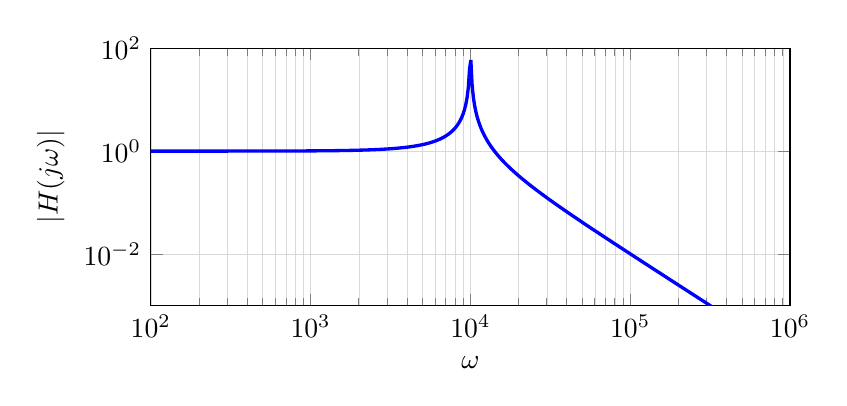
\begin{tikzpicture}[
    declare function={
    mag(\omega)= (10^8) / (sqrt((10^8 - \omega^2)^2 + (\omega * 100)^2))
    ;
    }
]
    \begin{loglogaxis}
    [
    ymin=0.001, ymax=100, ylabel=$|H(j\omega)|$,
    xmin=10^2, xmax=10^6, xlabel=$\omega$,
    domain=10^2:10^6,
    grid=both, grid style={line width=.1pt, draw=gray!30},
    width=\textwidth * 0.8,
    height=\textwidth / 2.5,
    samples=500
    ]
    \addplot [blue,very thick] {mag(x)};
    \end{loglogaxis}
\end{tikzpicture}
\end{center}

\section{Module 2}
% \section*{Midterm 1 Review}

\renewcommand{\arraystretch}{1.25}

\subsection*{State-space models of systems}
In this unit, we are focusing on taking real-world systems and then working with them as matrix-vector equations. The first step to doing this is to represent systems with \textbf{state-space models}. \\
\newline
There are two parts to coming up with a state-space model:
\begin{enumerate}
    \item \textit{Choosing state variables.} These are the quantities that will appear in the $\vec{x}$ vector in an equation like 
    $$\frac{d}{dt}\vec{x}(t) = A\vec{x}(t) + B\vec{u}(t)$$ 
    \item \textit{Finding a differential or recurrence relation involving state variables:} i.e. find $\frac{d}{dt} \vec{x}$ in terms of $\vec{x}$ for a continuous-time system or find $\vec{x}(k + 1)$ in terms of $\vec{x}(k)$ for a discrete-time system. \\
    \newline
    Typically, this consists of filling in the elements of the $A$ matrix and $B$ vector, such as in the following equation:
    \begin{align*}
        \vec{x}(k + 1) = \begin{bmatrix}
            a_{11} & a_{12} \\
            a_{21} & a_{22}
        \end{bmatrix} \vec{x}(k) + \begin{bmatrix} b_1 \\ b_2 \end{bmatrix} u(t)
    \end{align*}
    However, \textbf{non-linear systems} cannot be represented as matrix-vector equations, so the state-space model can look as follows:
    \begin{align*}
        \frac{d}{dt} \vec{x}(t) = \begin{bmatrix}
            x_1^{\,2} + \cos(x_2) \\
            x_1^{\,3} - \sin(x_2)
        \end{bmatrix}
    \end{align*}
\end{enumerate}
For instance, when you analyzed the LRC circuit, you chose the voltage across the capacitor and the current through the inductor as your state variables and then used the current-voltage relationships of capacitors and inductors to come up with the following state-space representation:
\begin{align*}
    \frac{d}{dt} \begin{bmatrix} 
        I_L(t) \\ V_C(t)
    \end{bmatrix} = \begin{bmatrix}
        -R/L & -1/L \\
        1/C & 0
    \end{bmatrix} \begin{bmatrix} 
        I_L(t) \\ V_C(t)
    \end{bmatrix}
    \end{align*}

\subsection*{Linearization}
Many systems in the real world are nonlinear, which means that we cannot represent them with a matrix-vector equation. 
We would like to use linear tools (such as diagonalization) to solve these equations, so we typically linearize nonlinear systems. \\
\newline
\textbf{When is a system linear?} \\
A system is linear if it follows the \textbf{scaling} and \textbf{additivity} properties:
\begin{enumerate}
    \item \textbf{Scaling}: For a linear system $f$, $f(ax) = af(x)$ for every $a$ and for every $x$.
    \item \textbf{Additivity}: For a linear system $f$, $f(x + y) = f(x) + f(y)$ for every $x, y$.
\end{enumerate}
\textit{Note: Equations of the form $f(x) = ax + b$ with nonzero $b$ are not linear; they are considered to be \textbf{affine}}. \\
\newline
\textbf{Linearizing a nonlinear system} \\
We convert a nonlinear system into a linear system by using a first-order Taylor approximation:
$$f(x) \approx f(x^*) + \frac{df}{dx} \bigg\rvert_{x = x^*} (x - x^*)$$
Or, for an equation with an input, $u$:
$$f(x, u) \approx f(x^*, u^*) + \frac{df}{dx} \bigg\rvert_{x = x^*} (x - x^*) + \frac{df}{du} \bigg\rvert_{u = u^*} (u - u^*)$$
In these equations, we linearize the system around an \textbf{equilibrium point} or \textbf{operating point}, $(x^*, u^*)$. 
This is a point that we choose when making our approximation, typically so that
$$f(x^*, u^*) = 0$$
\newline
\textbf{Linearizing a system of nonlinear equations} \\
Say we have a system of nonlinear functions, typically represented by
\begin{align*}
    \vec{f}(\vec{x}) = \begin{bmatrix}
        f_1(x_1, \dots, x_n) \\
        \vdots \\
        f_m(x_1, \dots, x_n)
    \end{bmatrix}
\end{align*}
For these systems, you can linearize each equation using the partial derivative of the function with respect to each state variable:
\begin{center}
    \begin{align*}
        f_1(\vec{x}) \approx f_1(\vec{x}^*) + \frac{\partial f_1}{\partial x_1} \bigg\rvert_{x_1 = x_1^*} (x_1 - x_1^*) + \cdots + \frac{\partial f_1}{\partial x_n} \bigg\rvert_{x_n = x_n^*} (x_n - x_n^*) \\
        \vdots \\
        f_m(\vec{x}) \approx f_m(\vec{x}^*) + \frac{\partial f_m}{\partial x_1} \bigg\rvert_{x_1 = x_1^*} (x_1 - x_1^*) + \cdots + \frac{\partial f_m}{\partial x_n} \bigg\rvert_{x_n = x_n^*} (x_n - x_n^*)
    \end{align*}
\end{center}
In this case, we choose an $\vec{x}^*$ and $\vec{u}^*$ such that $\vec{f}(\vec{x}^*, \vec{u}^*) = \vec{0}$. \\
\newline
We can express this linearization as a matrix-vector equation:
\begin{align*}
    \vec{f}(\vec{x}) = \begin{bmatrix}
        \frac{\partial f_1}{\partial x_1} \bigg\rvert_{x_1^*} & \cdots & \frac{\partial f_1}{\partial x_n} \bigg\rvert_{x_n^*} \\
        \vdots & \ddots & \vdots \\
        \frac{\partial f_m}{\partial x_1} \bigg\rvert_{x_1^*} & \cdots & \frac{\partial f_m}{\partial x_n} \bigg\rvert_{x_n^*}
    \end{bmatrix} \begin{bmatrix}
        (x_1 - x_1^*) \\
        \vdots \\
        (x_n - x_n^*)
    \end{bmatrix} = J_{\vec{x}} \vec{\delta x}
\end{align*}
Where $J_{\vec{x}}$ is the \textbf{Jacobian matrix} of $\vec{f}$ with respect to $\vec{x}$ and $\vec{\delta x}$ is the distance of $\vec{x}$ from the equilibrium point. \\
\newline
If we are looking at a system of equations with a vector input, the linearization will be as follows
\begin{align*}
    \vec{f}(\vec{x}, \vec{u}) = \begin{bmatrix}
        \frac{\partial f_1}{\partial x_1} \bigg\rvert_{x_1^*} & \cdots & \frac{\partial f_1}{\partial x_n} \bigg\rvert_{x_n^*} \\
        \vdots & \ddots & \vdots \\
        \frac{\partial f_m}{\partial x_1} \bigg\rvert_{x_1^*} & \cdots & \frac{\partial f_m}{\partial x_n} \bigg\rvert_{x_n^*}
    \end{bmatrix} \begin{bmatrix}
        (x_1 - x_1^*) \\
        \vdots \\
        (x_n - x_n^*)
    \end{bmatrix} + \begin{bmatrix}
        \frac{\partial f_1}{\partial u_1} \bigg\rvert_{u_1^*} & \cdots & \frac{\partial f_1}{\partial u_k} \bigg\rvert_{u_k^*} \\
        \vdots & \ddots & \vdots \\
        \frac{\partial f_m}{\partial u_1} \bigg\rvert_{u_1^*} & \cdots & \frac{\partial f_m}{\partial u_k} \bigg\rvert_{u_k^*}
    \end{bmatrix} \begin{bmatrix}
        (u_1 - u_1^*) \\
        \vdots \\
        (u_k - u_k^*)
    \end{bmatrix} = J_{\vec{x}} \vec{\delta x} + J_{\vec{u}} \vec{\delta u}
\end{align*}

\subsection*{Discretization}
Another modification we often make is converting systems from \textbf{continuous time} (represented by a \textit{differential equation}) to \textbf{discrete time} (represented by a \textit{recurrence relation}).
One motivation behind discretizing a system is that computers can only sample the system at discrete points in time, and can only provide piecewise constant inputs. \\
\newline
\textbf{Discretizing a system} \\
Let's say you have an differential equation of the form
$$\frac{d}{dt} x = f(t) + u(t)$$
We want to convert it into the discrete-time recurrence relation
$$\tilde{x}(k + 1) = a\tilde{x}(k) + \tilde{u}(k)$$
where $\tilde{x}(k)$ is the discrete-time counterpart of $x(t)$ and $\tilde{u}(k)$ is the discrete-time counterpart of the input $u(t)$.
\newline
We are given our system has time step $T$, which you can think of as having two implications:
\begin{enumerate}
    \item Inputs are constant between times $nT$ and $(n + 1)T$.
    \item When we discretize the system, $\tilde{x}(k) = x(kT)$.
\end{enumerate}
In order to discretize the system, we want to find $x(t + T)$ in terms of $x(t)$, assuming a constant input in the interval $[t, t + T)$.
To do so, you can integrate the system between $t$ and $t + T$:
\begin{align*}
    \int_{x(t)}^{x(t + T)} dx = \int_t^{t + T} (f(\tau) + u(\tau)) \, d\tau \\
\end{align*}
Note that the variable of integration on the right-hand side is $\tau$, not $t$ because $t$ is present in the limits of integration. \\
If $F$ is the antiderivative of $f$, we can get the following expression for $x(t + T)$
\begin{align*}
    x(t + T) = x(t) + (F(t + T) - F(t) + Tu(t))
\end{align*}
Now, we have the information we need to get $\tilde{x}(k + 1)$ in terms of $\tilde{x}(k)$ and $\tilde{u}(k)$. 
If we set $t = kT$, we have
\begin{align*}
    x((k + 1)T) = x(kT) + (F((k + 1)T) - F(kT) + Tu(kT)) \\
    \tilde{x}(k + 1) = \tilde{x}(k) + (F((k + 1)T) - F(kT) + Tu(kT))
\end{align*}
So, in the expression $\tilde{x}(k + 1) = a\tilde{x}(k) + \tilde{u}(k)$, $a = 1$ and $\tilde{u}(k) = F((k + 1)T) - F(kT) + Tu(kT)$.

\subsection*{Controllability}
We say that a system of the form
$$\vec{x}(k + 1) = A\vec{x}(k) + \vec{b} u(k)$$
is controllable if, given any $\vec{x}(0)$, we can specify a series of control inputs $(u(0), u(1), \dots, u(n))$ to reach any state (so, $\vec{x}(n)$ can be anything we want it to be). \\
To determine whether a system is controllable, we define its controllability matrix to be
\begin{align*}
    \mathcal{C} = \begin{bmatrix}
        \vec{b} & A\vec{b} & \cdots & A^{n - 1} \vec{b}
    \end{bmatrix}
\end{align*}
Assuming we start at $\vec{x}(0) = \vec{0}$, we can reach any state in the span of the columns of $\mathcal{C}$, and therefore the system is controllable if the $\mathcal{C}$ is \textbf{full rank}, i.e., for an n-dimensional $\vec{x}$, the controllability matrix has n linearly independent columns. \\
\newline
\textbf{Controlling a system} \\
Assume we have a scalar input $u(k)$ and we want to see what states we can reach with $n$ controls if we start at $\vec{x}(0) = \vec{0}$. \\ 
\newline
Plugging the controls into the recurrence relation, we see that the first column of the controllability matrix corresponds to the last input ($u(n - 1)$), the second column corresponds to the second-to-last input ($u(n - 2)$), and the $n^{\text{th}}$ column corresponds to $u(0)$: 
\begin{align*}
    \vec{x}(n) = A\vec{x}(n - 1) + \vec{b} u(n - 1) \\
    \vec{x}(n) = A(A \vec{x}(n - 2) + \vec{b} u(n - 2)) + \vec{b} u(n - 1) \\
    = A^2 \vec{x}(n - 2) + A\vec{b} u(n - 2) + \vec{b} u(n - 1) \\
    \cdots
    \vec{x}(n) = A^n \vec{x}(0) + A^{n - 1} \vec{b} u(0) + \cdots +  A\vec{b} u(n - 2) + \vec{b} u(n - 1) \\
    = A^{n - 1} \vec{b} u(0) + \cdots +  A\vec{b} u(n - 2) + \vec{b} u(n - 1)
\end{align*}
So, if we want to pick control values such that a system reaches a certain $\vec{x}(n)$ starting at $\vec{x}(0) = \vec{0}$, we can use the relation
\begin{align*}
    \vec{x}(n) = \mathcal{C} \begin{bmatrix}
        u(n - 1) \\ \vdots \\ u(0)
    \end{bmatrix}
\end{align*}
and solve for your control inputs as follows:
\begin{align*}
    \begin{bmatrix}
        u(n - 1) \\ \vdots \\ u(0)
    \end{bmatrix} = \mathcal{C}^{-1} \vec{x}(n)
\end{align*}

\subsection*{System Identification}
If we don't know the parameters of our system (i.e. the $A$ matrix and $\vec{b}$ vector) but we do have a series of inputs and outputs to the system, we can use least squares to solve for the elements of $A$ and $\vec{b}$. \\
\newline
First, let us consider a 2-dimensional system with a scalar input.
\begin{align*}
    \begin{bmatrix}
        x_1(k + 1) \\ x_2(k + 1)
    \end{bmatrix} = \begin{bmatrix}
        a_{11} & a_{12} \\
        a_{21} & a_{22}
    \end{bmatrix} \begin{bmatrix}
        x_1(k) \\ x_2(k)
    \end{bmatrix} + \begin{bmatrix}
        b_1 \\ b_2
    \end{bmatrix} u(k)
\end{align*}
Also, let's say we are given the following data points: $\vec{x}(0), \dots, \vec{x}(m)$ and $u(0), \dots, u(m - 1)$. \\
\newline
In order to perform system identification, we want to format the system as a least squares problem:
\begin{align*}
    D\vec{p} \approx \vec{y}
\end{align*}
$\vec{p}$ is our vector of unknowns, so we populate it with the elements of $A$ and $\vec{b}$:
\begin{align*}
    \vec{p} = \begin{bmatrix}
        a_{11} & a_{12} & a_{21} & a_{22} & b_1 & b_2
    \end{bmatrix}^T
\end{align*}
We can view $\vec{y}$ as the output of the system, so we can populate with $\vec{x}(1), \dots, \vec{x}(m)$
\begin{align*}
    \vec{y} = \begin{bmatrix}
        x_1(1) & x_2(1) & \cdots & x_1(m) & x_2(m)
    \end{bmatrix}^T
\end{align*}
Now, we need to find the elements of the $D$ matrix to complete the relationship between $\vec{p}$ and $\vec{y}$. 
From the matrix-vector representation of the system, we get scalar equations of the form
\begin{align*}
    x_1(k + 1) = a_{11} x_1(k) + a_{12} x_2(k) + b_1 u(k) \\
    x_2(k + 1) = a_{21} x_1(k) + a_{22} x_2(k) + b_2 u(k) 
\end{align*}
So, we have the following least-squares problem:
\begin{align*}
    \begin{bmatrix}
        x_1(1) \\ x_2(1) \\ x_1(2) \\ x_2(2) \cdots \\ x_1(m) \\ x_2(m)
    \end{bmatrix} = \begin{bmatrix}
        x_1(0) & x_2(0) & 0 & 0 & u(0) & 0 \\
        0 & 0 & x_1(0) & x_2(0) & 0 & u(0) \\
        x_1(1) & x_2(1) & 0 & 0 & u(1) & 0 \\
        0 & 0 & x_1(1) & x_2(1) & 0 & u(1) \\
        \vdots & \vdots & \vdots & \vdots & \vdots & \vdots \\
        x_1(m - 1) & x_2(m - 1) & 0 & 0 & u(m - 1) & 0 \\
        0 & 0 & x_1(m - 1) & x_2(m - 1) & 0 & u(m - 1)
    \end{bmatrix} \begin{bmatrix}
        a_{11} \\ a_{12} \\ a_{21} \\ a_{22} \\ b_1 \\ b_2
    \end{bmatrix}
\end{align*}
From here, we can solve for $\vec{p}$ using the least-squares formula:
$$\vec{p} = (D^T D)^{-1} D^T \vec{y}$$
This also extrapolates to systems of higher dimension.
\newline
\textit{Note: At the very least, you need $\vec{x}(0), \dots \vec{x(3)}$ and $u(0), u(1), u(2)$ because we have 6 unknowns and need 6 equations to have a unique solution.}

\subsection*{SVD}

\section{Module 3}
\renewcommand{\arraystretch}{1.25}

\subsection*{Applications of the SVD}
\textbf{Principal Component Analysis}

\textit{Principal Component Analysis} (PCA) is a procedure that uses the SVD to analyze data by finding the directions of maximum "spread" or variation. Some of its uses include visualizing high dimensional data and revealing patterns that are useful to perform classification.\\
\newline
Below, we show the steps of performing PCA, as well as visualizations on a two dimensional dataset:

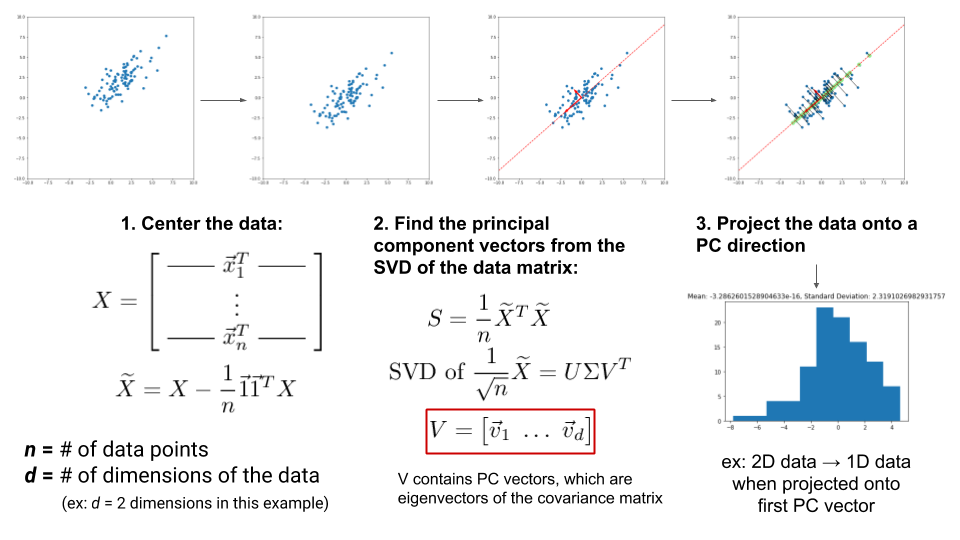
\includegraphics[width=\textwidth]{figures/pca-steps}

In summary,
\begin{enumerate}
    \item We first \textbf{de-mean} the data. If the each datapoint is represented as a \textit{row}, then we are going to want find the mean of each \textit{column} and subtract it from each element in that \textit{column} to make it \textbf{zero-mean}. If each datapoint is a \textit{column}, we want every \textit{row} to be zero-mean.
    \item If each datapoint is a \textit{row} (which this example assumes), the covariance matrix is $\frac{1}{n} \widetilde{X}^T\widetilde{X}$, and the \textit{principal components are the columns of $V$} in the SVD (eigenvectors of the covariance matrix). 
    If each datapoint is a \textit{column}, the covariance matrix is $\frac{1}{m} \widetilde{X}\widetilde{X}^T$, and the \textit{principal components correspond to the columns of $U$}. \\
    \newline
    You can think of the covariance matrix as measuring the relation between the quantities we're measuring, and its eigenvectors as the directions in our data with the most variation.
    \item When you have the principal components, you can \textbf{project datapoints onto the principal components} to see how much of each principal component contributes to that datapoint.
\end{enumerate}

\newpage
\textbf{Minimum Norm Control} \\
Say we have a controllable system of rank $n$
\begin{align*}
    \vec{x}(k + 1) = A\vec{x}(k) + \vec{b}u(k)
\end{align*}
 and we want to reach a desired state $\vec{x}_f$ with $k > n$ control inputs. We know we can reach any state in $n$ timesteps, and there are infinitely many ways to reach $\vec{x}_f$ in $k > n$ timesteps. Using the SVD, however, we can find the series of control inputs that has the minimum norm. \\
 \newline
 Recall from the section on control that we can use the following linear system to solve for the control inputs:
 \begin{align*}
    \vec{x}(k) = \mathcal{C}_k \begin{bmatrix}
        u(k - 1) \\ \vdots \\ u(0)
    \end{bmatrix} \\
    \vec{x}(k) = \begin{bmatrix}
        \vec{b} & A\vec{b} & \cdots & A^{k - 1} \vec{b}
    \end{bmatrix} \begin{bmatrix}
        u(k - 1) \\ \vdots \\ u(0)
    \end{bmatrix}
 \end{align*}

To solve for the minimum norm solution, we use the \textbf{Moore-Penrose Pseudoinverse}, a generalization of matrix inverses for rectangular matrices using the full SVD of a matrix. We denote the pseudoinverse with a dagger, and the solution will be $\vec{x} = A^{\dagger} \vec{b}.$ (\textit{Note: in the case of finding control inputs, you would replace $A$ with $\mathcal{C}_k$})
This solution is special in that it has \textbf{minimum norm.} That is, if we have another solution $\vec{z},$ such that $A \vec{z} = \vec{b},$ then $\norm{x} \leq \norm{z}.$

To compute the pseudoinverse, we invert each element of the SVD one at a time:

\begin{align*}
    A \vec{x} &= \vec{y} \\
    U \Sigma V^T \vec{x} &= \vec{y} \\
    (U^T U) \Sigma V^T \vec{x} &= U^T \vec{y} \\
    (\Sigma^{\dagger} \Sigma) V^T \vec{x} &= \Sigma^{\dagger} U^T \vec{y} \\
    (V V^T) \vec{x} &= V \Sigma^{\dagger} U^T \vec{y} \\
    \vec{x} &= V \Sigma^{\dagger} U^T \vec{y} \\
    \implies \vec{x} &= A^{\dagger} \vec{y}
\end{align*}

We can calculate $\Sigma^{\dagger}$ accordingly to produce an identity matrix so that the term $\Sigma^{\dagger}\Sigma$ disappears.

$$\Sigma^{\dagger} = \begin{bmatrix} \frac{1}{\sigma_{1}} & 0 &  \cdots & 0 \\ 0 & \frac{1}{\sigma_{2}} & \cdots & 0 \\ \vdots & \vdots & \ddots & \frac{1}{\sigma_{m}} \\ 
    \vdots & \vdots & \ddots & 0 \\ 0 & 0 & 0 & 0 \end{bmatrix}$$

\textit{Note}: another, sometimes computationally easier, form of the pseudoinverse for wide matrices is:
$$\vec{x} = A^T(AA^T)^{-1}\vec{y}$$
(See Sp20 Note 11B for more information)

\subsection*{Stability}
A continuous- or discrete-time system is considered \textit{stable} if, for any bounded initial condition and series of inputs, the state remains bounded (if a quantity is \textit{bounded}, it is less than some finite constant at all times). We sometimes refer to this as BIBO (bounded input implies bounded output) stability. \\
\newline
For a system in \textit{discrete time}
$$\vec{x}(k + 1) = A\vec{x}(k) + \vec{b}u(k)$$
The system is
\begin{enumerate}
    \item \textbf{Stable} if all eigenvalues have a \textbf{magnitude less than 1},
    \item \textbf{Unstable} if at least one eigenvalue has a \textbf{magnitude greater than 1}, or
    \item \textbf{Marginally unstable} if at least one eigenvalue has a magnitude of 1 and none have a magnitude greater than 1.
\end{enumerate}

For a system in \textit{continuous time}
$$\frac{d}{dt} \vec{x}(t) = A\vec{x}(t) + \vec{b}u(t)$$
The system is
\begin{enumerate}
    \item \textbf{Stable} if all eigenvalues have a \textbf{negative real component},
    \item \textbf{Unstable} if at least one eigenvalue has a \textbf{positive real component}, or
    \item \textbf{Marginally unstable} if at least one eigenvalue has a real component of 0 and none have a positive real component.
\end{enumerate}

If we plot the eigenvalues on the \textit{complex plane}, a \textbf{discrete-time system} is stable if all eigenvalues are \textbf{strictly inside the unit circle} (left graph), and a \textbf{continuous-time system} is stable if all eigenvalues are on the left half of the plane (right graph): \\
\begin{tabular}{p{0.5\textwidth} p{0.5\textwidth}}
    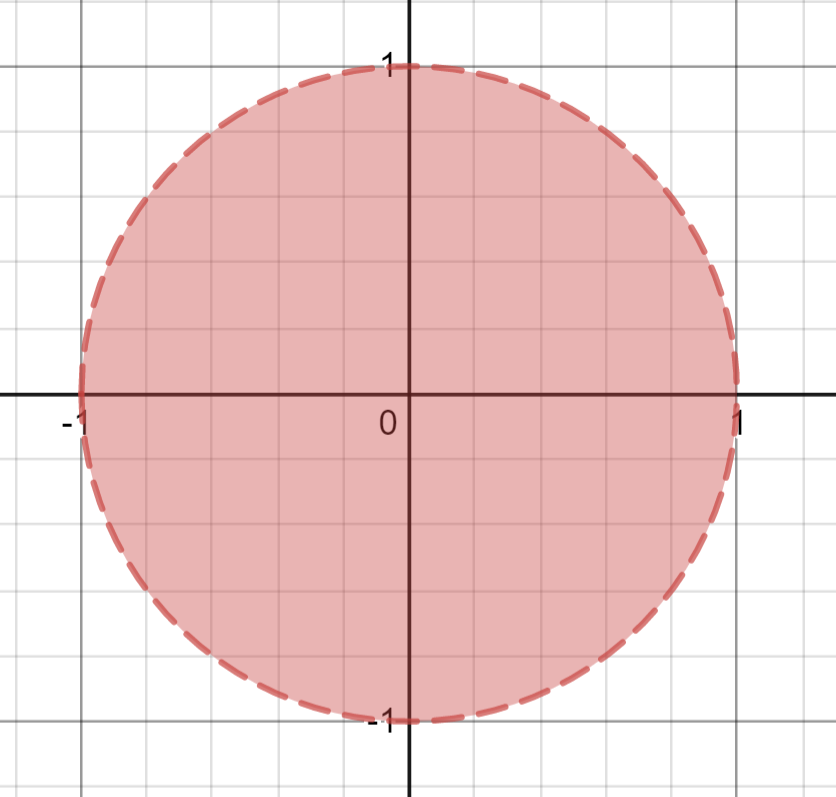
\includegraphics[width = 0.35 \textwidth]{\bank/../sp20/final/figures/discrete-stable.PNG} & 
    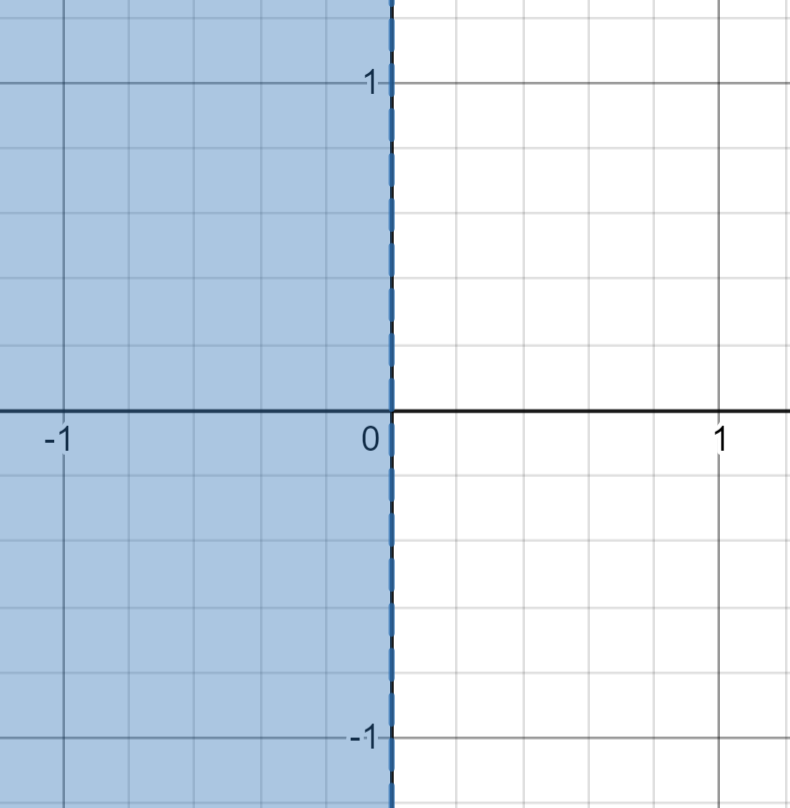
\includegraphics[width = 0.35 \textwidth]{\bank/../sp20/final/figures/continuous-stable.PNG}
\end{tabular}

An interesting case is \textit{upper-triangular matrices}. If a matrix is upper-triangular, its eigenvalues are on the diagonal. So, to see if a system with an upper-triangular A matrix is stable, you can look at the diagonal elements. \\
\newline

\textbf{Visualizing stability}: \\
We know that stable eigenvalues cause any input or initial condition to decay over time, unstable eigenvalues cause the state to grow exponentially, and marginally unstable eigenvalues cause any disturbance to neither decay nor grow. 
In addition, whether or not the eigenvalues have a complex component determines whether the state oscillates (continuous time), or rotates (discrete time). \\
\newline
The following plots will explore how complex eigenvalues affect the state evolution of stable and unstable systems.

\begin{tabular}{|p{0.3\textwidth}| p{0.3\textwidth}|b{0.4\textwidth}|}
    \multicolumn{3}{c}{Plots of $\vec{x}_1(k)$ for discrete-time systems with initial condition $\begin{bmatrix} 1 & 1 \end{bmatrix}^T$} \\
    \hline
    Real and Positive $\lambda$ & Complex or Negative $\lambda$ & Description \\
    \hline & & \\
    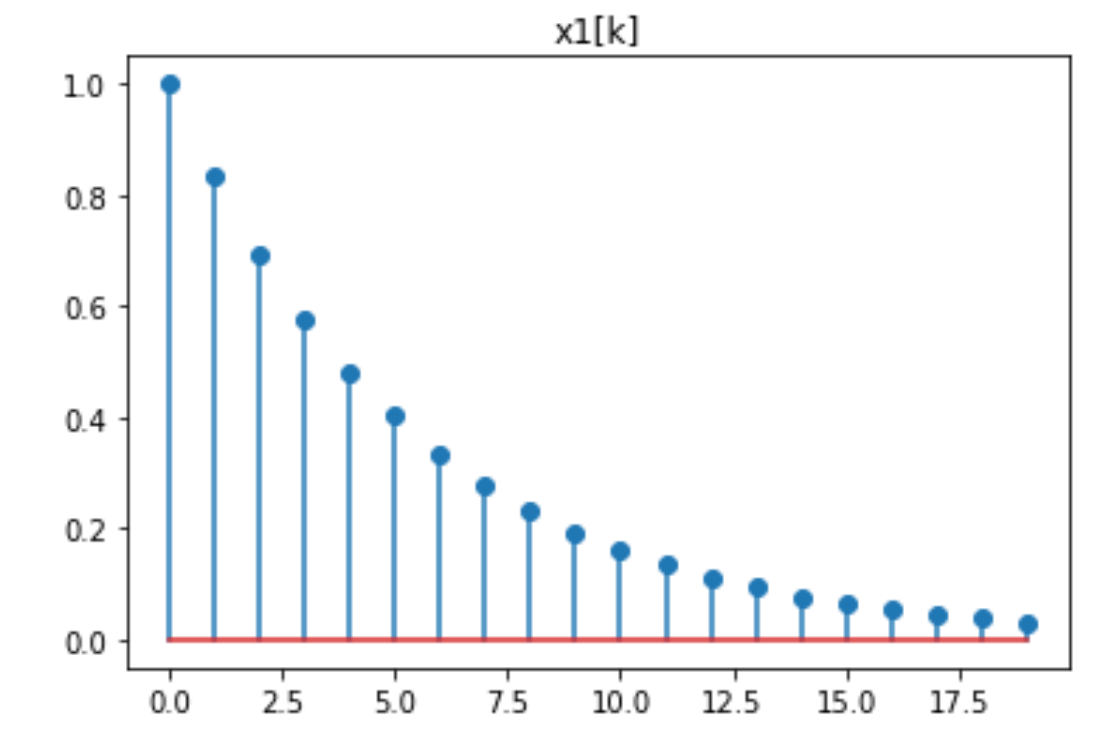
\includegraphics[width = 0.3 \textwidth]{\bank/stability/figures/discrete-graphs/stable-real-x1.PNG} &
    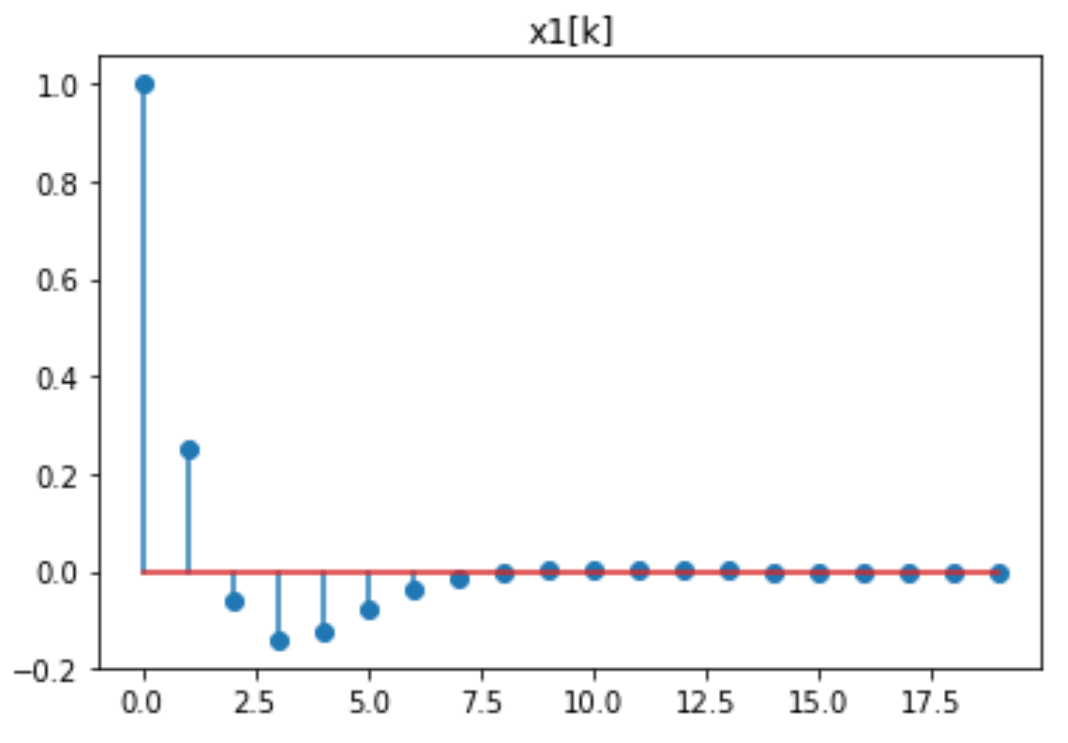
\includegraphics[width = 0.3 \textwidth]{\bank/stability/figures/discrete-graphs/stable-complex-x1.PNG} &
    \textbf{Stable system}: The system is stable, so the initial condition decays over time. When the eigenvalues are \textbf{real}, there is \textbf{no rotation}, but when they are \textbf{complex}, the state vector \textbf{rotates each timestep}. \\
    \hline & & \\
    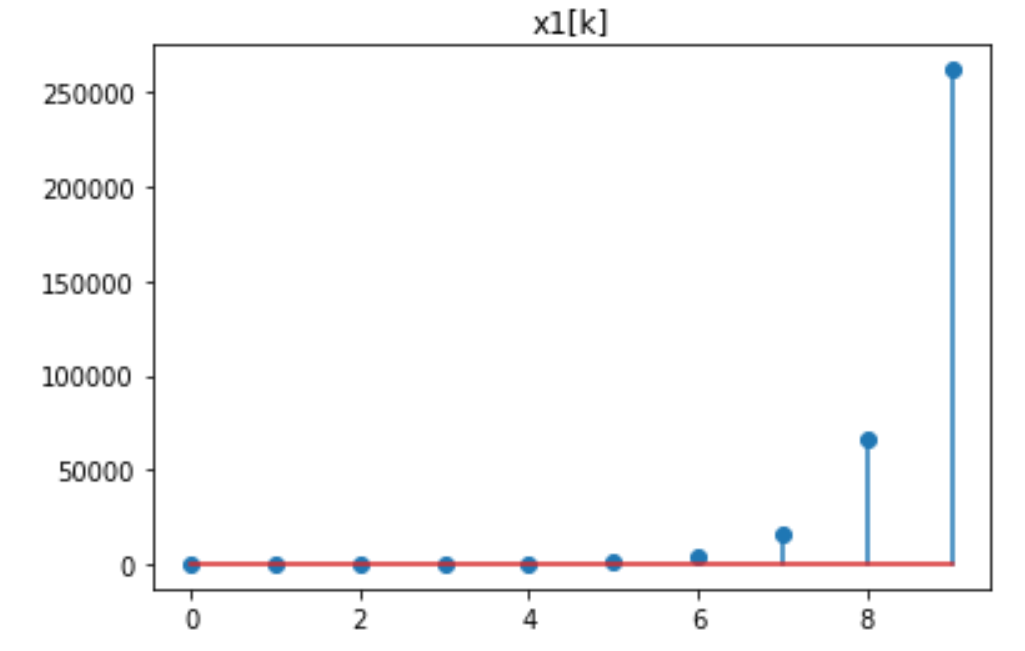
\includegraphics[width = 0.3 \textwidth]{\bank/stability/figures/discrete-graphs/unstable-real-x1.PNG} &
    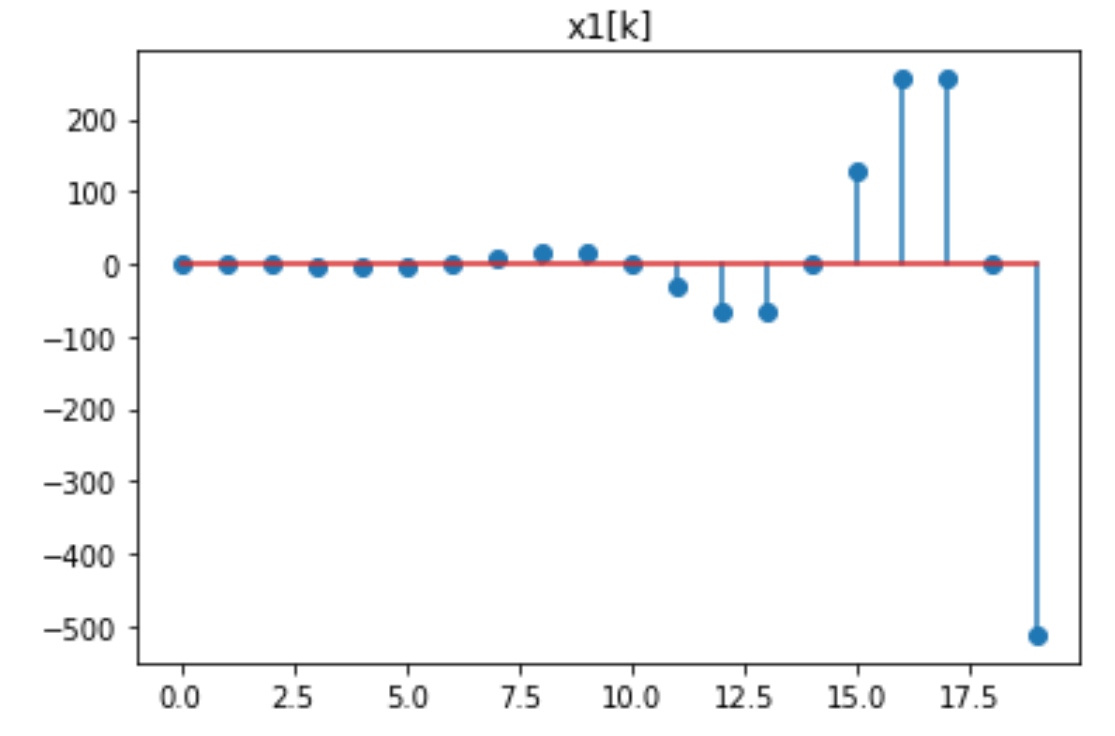
\includegraphics[width = 0.3 \textwidth]{\bank/stability/figures/discrete-graphs/unstable-complex-x1.PNG} &
    \textbf{Unstable system}: The system is unstable, so the initial condition grows exponentially. The state vector rotates only when the eigenvalues are complex. \\
    \hline & & \\
    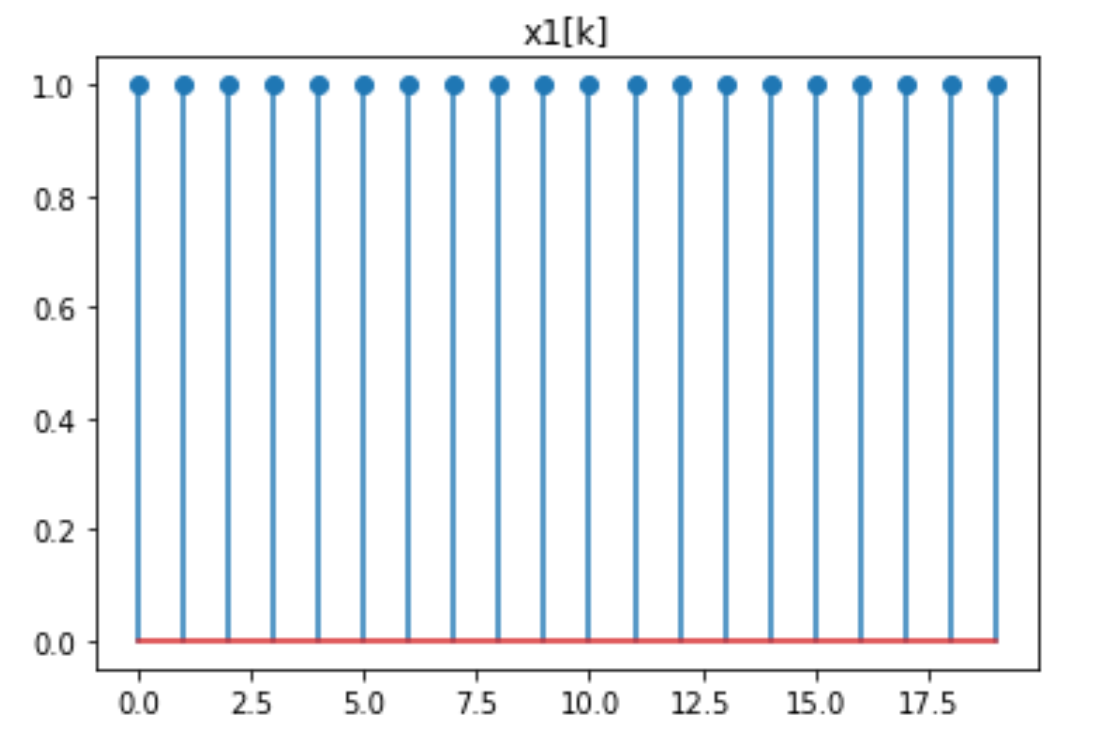
\includegraphics[width = 0.3 \textwidth]{\bank/stability/figures/discrete-graphs/marginal-real-x1.PNG} &
    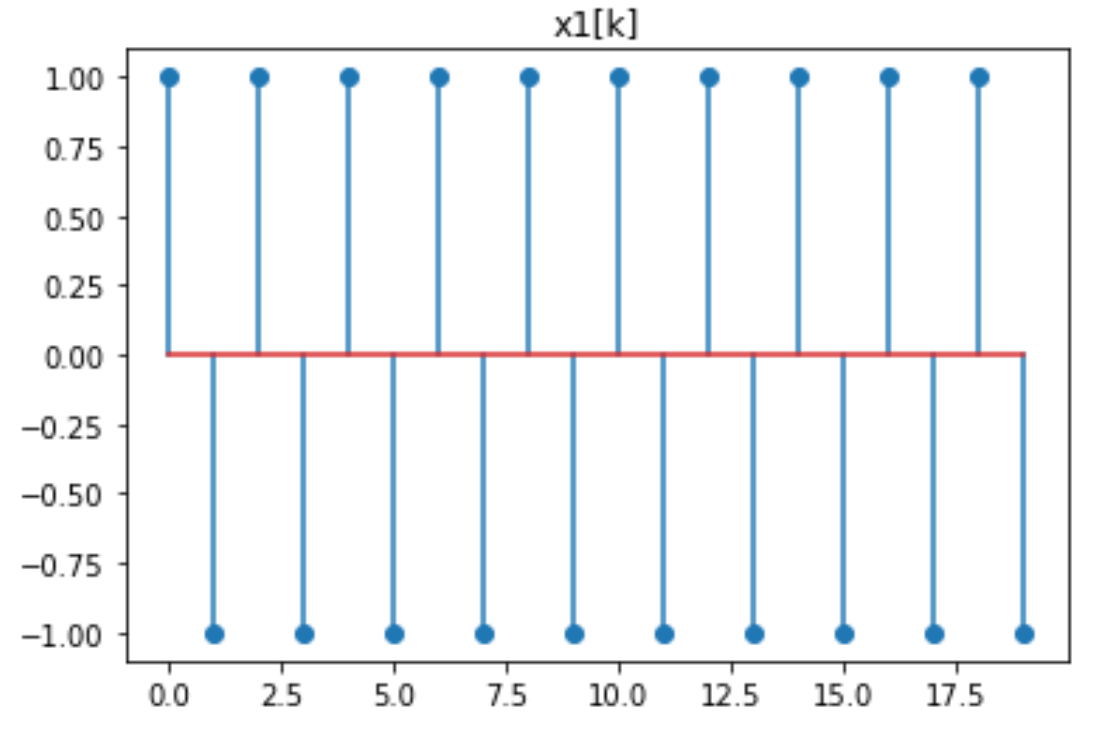
\includegraphics[width = 0.3 \textwidth]{\bank/stability/figures/discrete-graphs/marginal-negative-x1.PNG} &
    \textbf{Marginally unstable}: The initial condition neither grows nor decays. When both eigenvalues are 1, the state vector stays constant. When the eigenvalues are elsewhere on the unit circle, the state vector rotates.\\
    \hline
\end{tabular}

\begin{tabular}{|p{0.3\textwidth}| p{0.3\textwidth}|b{0.4\textwidth}|}
     \multicolumn{3}{c}{Plots of $\vec{x}_1(t)$ for continuous-time systems with initial condition $\begin{bmatrix} 1 & 1 \end{bmatrix}^T$} \\
    \hline
    Real $\lambda$ & Complex or Imag. $\lambda$ & Description \\
    \hline & & \\
    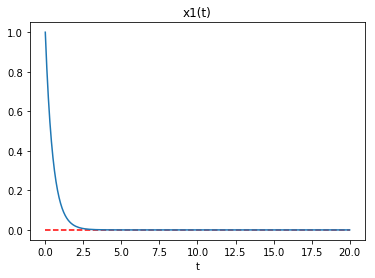
\includegraphics[width = 0.3 \textwidth]{\bank/stability/figures/continuous-graphs/real_negative_x1.png} &
    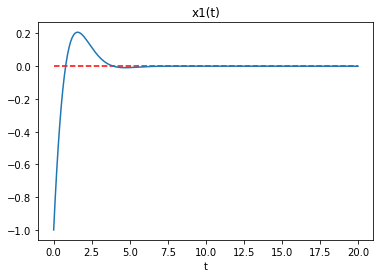
\includegraphics[width = 0.3 \textwidth]{\bank/stability/figures/continuous-graphs/complex_negative_x1.png} &
    \textbf{Stable system}: The system is stable, so the initial condition decays over time. When the eigenvalues are \textbf{real}, there is \textbf{no oscillation}, but when they are \textbf{complex}, the state \textbf{oscillates}. \\
    \hline & & \\
    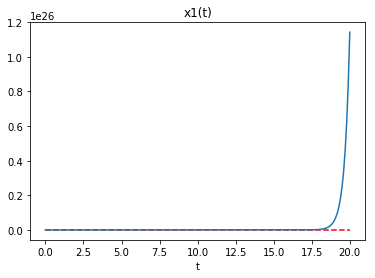
\includegraphics[width = 0.3 \textwidth]{\bank/stability/figures/continuous-graphs/real_positive_x1.png} &
    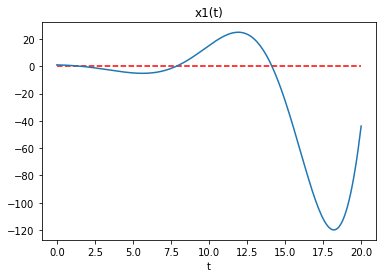
\includegraphics[width = 0.3 \textwidth]{\bank/stability/figures/continuous-graphs/complex_positive_x1.png} &
    \textbf{Unstable system}: The system is unstable, so the initial condition grows exponentially. The state oscillates only when the eigenvalues are complex. \\
    \hline & & \\
    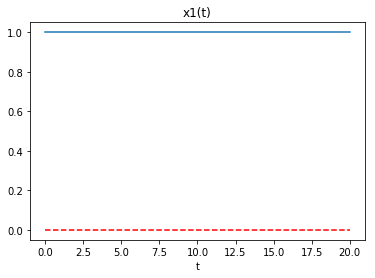
\includegraphics[width = 0.3 \textwidth]{\bank/stability/figures/continuous-graphs/zero_x1.png} &
    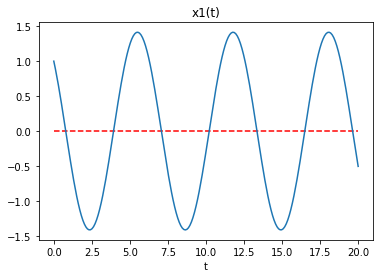
\includegraphics[width = 0.3 \textwidth]{\bank/stability/figures/continuous-graphs/imaginary_x1.png} &
    \textbf{Marginally unstable}: The initial condition neither grows nor decays. When both eigenvalues are 0, the state vector stays constant. When the eigenvalues are imaginary, the state oscillates without decaying.\\
    \hline
\end{tabular}


\subsection*{Feedback Control and Eigenvalue Placement}
Consider a system that is controllable but has unstable eigenvalues:
\begin{align*}
    \vec{x}(k + 1) = A\vec{x}(k) + \vec{b}u(k)
\end{align*}
We can use the fact that the system is controllable to place its eigenvalues wherever we want by applying a \textit{feedback control}, where the control input depends on the current state. Depending on the problem, the feedback input will either be of the form $u(t) = \vec{f^T} \vec{x}(k)$ or $u(t) = -\vec{f^T} \vec{x}(k)$. We will use the first in this worksheet, but you should expect to see both forms.
\begin{align*}
    \vec{x}(k + 1) = A\vec{x}(k) + \vec{b}\vec{f}^T \vec{x}(k)
\end{align*}
We can rewrite this system as follows:
\begin{align*}
    \vec{x}(k + 1) = (A + \vec{b}\vec{f}^T) \vec{x}(k)
\end{align*}
So, the new state transition matrix for the system is $(A + \vec{b}\vec{f}^T)$. Because the system is controllable, we can pick the elements of the feedback coefficient vector $\vec{f}$ to place the eigenvalues of our system wherever we choose. \\
\newline

\subsection*{CCF}
It is feasible to calculate feedback control coefficients by hand for a $2 \times 2$ system, but it quickly becomes difficult for higher-order systems. For systems in \textit{controller canonical form (CCF)}, however, it is a lot easier to apply feedback control. \\
\newline
In general, a system in CCF will look like the following:
\begin{align*}
    \vec{x}(k + 1) = \begin{bmatrix}
        0 & 1 & 0 & \cdots & 0 \\
        0 & 0 & 1 & \cdots & 0 \\
        \vdots & \vdots & \vdots & \ddots & \vdots \\
        0 & 0 & 0 & \cdots & 1 \\
        a_1 & a_2 & a_3 & \cdots & a_n
    \end{bmatrix} \vec{x}(k) + \begin{bmatrix}
        0 \\ 0 \\ \vdots \\ 0 \\ 1
    \end{bmatrix} u(k)
\end{align*}
For a system in CCF, the $B$ vector will be \textit{all zeros with a one in the last position}, and $A$ matrix will have \textit{ones in the position to the right of the diagonal and will be zero elsewhere, except in the last row}. \\
\newline
The interesting part about CCF is that the coefficients in the last row of the $A$ matrix \textbf{form the characteristic polynomial of our system}. 
For the above system, the characteristic polynomial would be:
\begin{align*}
    \lambda^n - a_n \lambda^{n - 1} - a_{n - 1}\lambda^{n - 2} - \cdots - a_2 \lambda - a_1 = 0
\end{align*}
Notice that each term after $\lambda^n$ is being \textit{subtracted}, and that the coefficients in the last row of $A$ are ordered in increasing rank (the constant term, then the coefficient of $\lambda$, etc). \\
\newline
Now, let's try to apply a feedback control input to see how useful CCF is.
\begin{align*}
    u(k) = \begin{bmatrix}
        f_1 & \cdots & f_n
        \end{bmatrix} \vec{x} \\
    \vec{x}(k + 1) = \begin{bmatrix}
        0 & 1 & 0 & \cdots & 0 \\
        0 & 0 & 1 & \cdots & 0 \\
        \vdots & \vdots & \vdots & \ddots & \vdots \\
        0 & 0 & 0 & \cdots & 1 \\
        a_1 & a_2 & a_3 & \cdots & a_n
    \end{bmatrix} \vec{x}(k) + \begin{bmatrix}
        0 \\ 0 \\ \vdots \\ 0 \\ 1
    \end{bmatrix} \begin{bmatrix}
        f_1 & \cdots & f_n
        \end{bmatrix} \vec{x}(k)
\end{align*}
The new state transition matrix would be the following:
\begin{align*}
    \begin{bmatrix}
        0 & 1 & 0 & \cdots & 0 \\
        0 & 0 & 1 & \cdots & 0 \\
        \vdots & \vdots & \vdots & \ddots & \vdots \\
        0 & 0 & 0 & \cdots & 1 \\
        a_1 & a_2 & a_3 & \cdots & a_n
    \end{bmatrix} \vec{x}(k) + \begin{bmatrix}
        0 \\ 0 \\ \vdots \\ 0 \\ 1
    \end{bmatrix} \begin{bmatrix}
        f_1 & \cdots & f_n
        \end{bmatrix} = \begin{bmatrix}
        0 & 1 & 0 & \cdots & 0 \\
        0 & 0 & 1 & \cdots & 0 \\
        \vdots & \vdots & \vdots & \ddots & \vdots \\
        0 & 0 & 0 & \cdots & 1 \\
        a_1 + f_1 & a_2 + f_2 & a_3 + f_3 & \cdots & a_n + f_n
    \end{bmatrix}
\end{align*}
And the new characteristic polynomial would be:
\begin{align*}
    \lambda^n - (a_n + f_n)\lambda^{n - 1} - \cdots - (a_2 + f_2) \lambda - (a_1 + f_1)
\end{align*}
As you can see, we can easily set the coefficients of the characteristic polynomial and therefore place the eigenvalues of the system. \\
\newline
% \textbf{CCF transformation and intuition (de-emphasized but in scope)}: \\
% In order to go from an arbitrary \textit{controllable} system to CCF, you can apply the transformation
% $$T = $$

\end{document}
